\chapter{Termo de Abertura do projeto}

\section{EAP}
\begin{figure}[!htb]
    \center{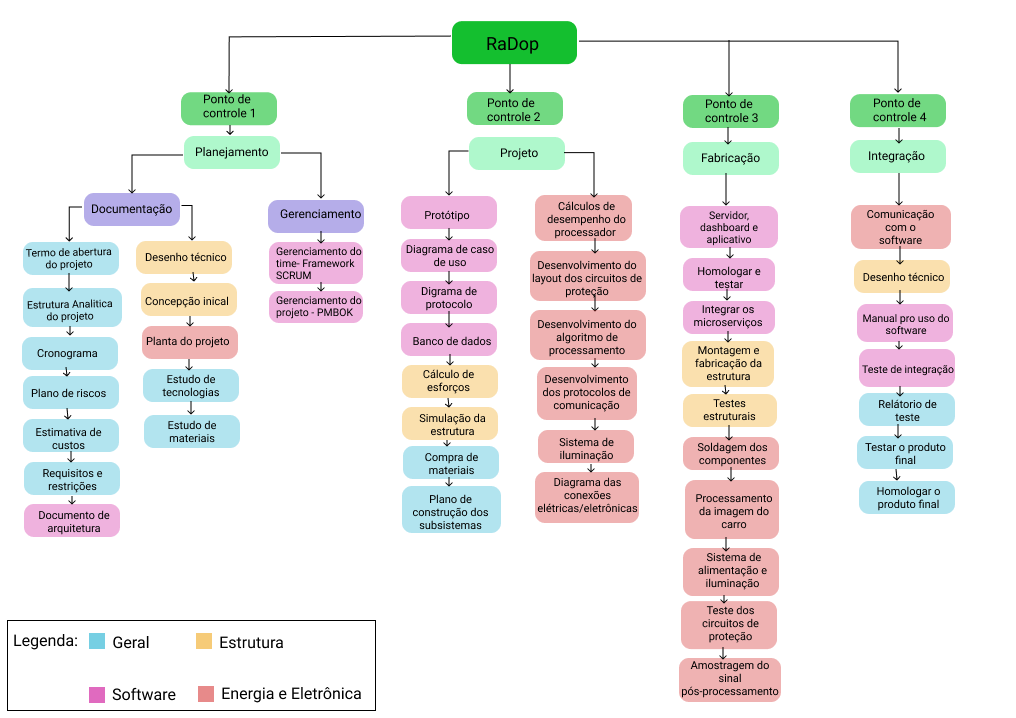
\includegraphics[width=\textwidth]{eap}}
    \caption{\label{fig:eap} EAP do projeto}
\end{figure}
\section{Lista É/Não é}
\subsection{É}
\subsection{Não é}
\section{Requisitos}
\subsection{Eletrônica}

Os requisitos de eletrônica são:
	
\begin{itemize}
	\item Detectar a aproximação do carro na via;
    \item Calcular a velocidade relativa do carro;
    \item Implementar uma comunicação entre os dois radares para determinar a emissão do alerta;
    \item Criar uma interface entre o radar e o motorista para visualização do alerta;
    \item Capturar imagem traseira do carro com a placa quando este passar acima da velocidade permitida;
    \item Projetar e construir circuitos de proteção para o dispositivos eletrônicos;
    \item Fazer o pré-processamento da imagem para reconhecimento da placa do veículo;
    \item Determinar a velocidade máxima do veículo para melhor captura da placa;
    \item Determinar a distância do veículo em relação ao radar para melhor captura da placa;
    \item Determinar a distância máxima entre os dois radares;
    \item Selecionar e implementar os protocolos de comunicação entre os dois radares;
    \item Selecionar e implementar os protocolos de comunicação entre os radares e o servidor;
     \item Determinar a capacidade de amarzenamento mínimo necessário para guardar dados quando a comunicação entre o radar e o servidor estiver fora de serviço;
     \item Determinar a velocidade mínima de transmissão de dados entre os radares para emissão de alerta;
     \item Determinar e implementar a estrutura do pacote de dados a ser enviado para o servidor contendo todas as informações necessárias;
     \item Transmitir para o servidor a velocidade, a imagem da placa pré-processada  e outras informações sobre o funcionamento do sistema.
\end{itemize}    
    
    As restrições de eletrônica são:

\begin{itemize}

	\item Se limitar em apenas reconhecer a placa do veículo, e não gerar a multa.
	\item Falha de comunicação entre os radares e o servidor por no máximo 3 dias.
	\item O veículo deve estar em uma velocidade igual ou menor que a velocidade máxima estabelecida para captura da placa.
	\item A captura da câmera deve ser apenas da traseira do veículo, devido a moto ter placa apenas na parte de trás, unificando o processo.
	\item A distância máxima entre os radares deve ser de 1 km.
	
\end{itemize} 	
	
\subsection{Energia}
\begin{itemize}
	\item O sistema deve conter painéis fotovoltaicos que promoverão a fonte de alimentação para todos os componentes do sistema;
	\item O sistema deve garantir o máximo aproveitamento energético;
	\item O sistema deve conter circuitos de controle de tensão e corrente;
	\item O sistema deve conter circuitos de controle de tensão e corrente;
	\item O sistema deve garantir o funcionamento seguro e contínuo do Radar;
	\item O sistema deve conter um circuito de iluminação para servir de alerta aos motoristas;

\end{itemize}

\subsubsection{Restrições}
\begin{itemize}
   \item Dependêcia do clima para a geração de energia;
   \item Localização Geografica;
   \item Temperatura média;
   \item Indices de radiação solar;
   \item Posicionamento das placas em relação a radiação solar;
   \item Horário de exposição;
   \item Existência de sombramento
 \end{itemize}
\subsection{Estrutura}
\subsection{Software}

Os requisistos de software são:

\begin{itemize}
    \item Interface do Dashboard;
    \item Interface do Aplicativo;
    \item Manual de uso dos softwares (Microsserviços, Aplicativo e Dashboard);
    \item Funcionar com conexão a redes (Internet);
    \item Ser capaz de lidar e recuperar de falhas e erros (conexão, processamento e etc.);
    \item Softwares devem ser manuteníveis e evolutíveis;
    \item Softwares devem ser testáveis e testados;
    \item Software deve mostrar dados e informações do Radar;
    \item Software deve ser capaz de tomar decisões para alertar socorristas a respeito de prováveis acidentes automobilísticos;
    \item Software deve ser capaz de tomar decisões para alertar usuários de possíveis situações de risco;
    \item Software deve ser capaz de mostrar informações gerenciais com os dados do Radar;
\end{itemize}

As restrições de software são:

\begin{itemize}
    \item O software necessita estar sempre conectado à internet para comunicação e, consequentemente, para o correto funcionamento;
    \item O aplicativo de manutenção irá auxiliar apenas com o essencial;
    \item O aplicativo só funcionará em aparelhos Android;
    \item A linguagem de cada microsserviço (assim como framework/tecnologia) será definida dada necessidade (performance, armazemanento e etc) dos mesmos;
\end{itemize}

\section{\emph{Stakeholders}}
\section{Recurso humanos}

 De modo a ter uma melhor organização, a equipe foi dividida em subgrupos, onde cada subgrupo tem um gerente técnico, além disso a equipe também conta com um gerente de qualidade e um coordenador geral. Na Figura \ref{fig:organograma} mostra o organograma da equipe e o nome de cada integrante por função.
 
\begin{figure}[h]
\centering
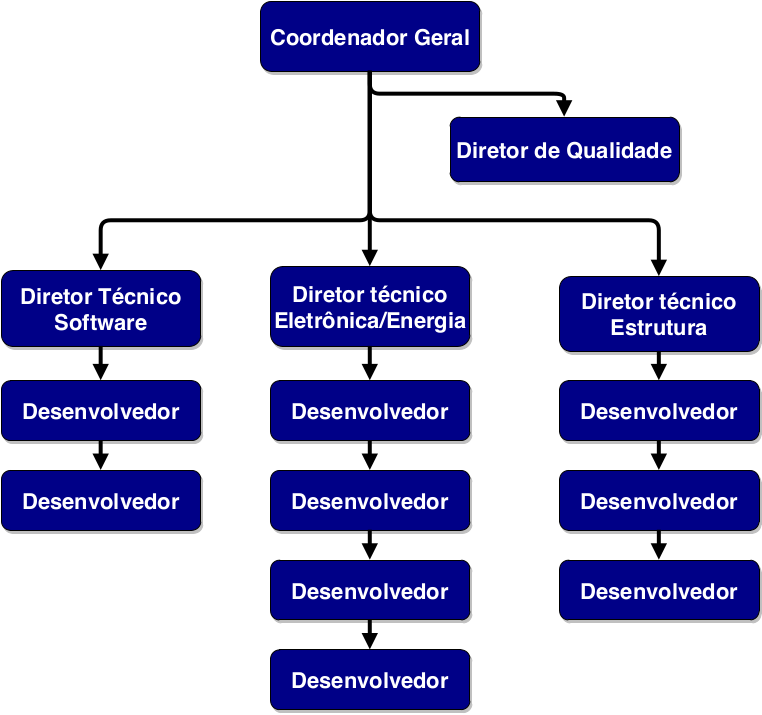
\includegraphics[scale = 0.5]{organograma.pdf}
\caption{.}\label{fig:organograma}
\end{figure} 

A seguir estão os nomes de cada integrante separado por área:

\begin{itemize}
\item Eletrônica e Energia

-Brenda Bianca Neves Dias\\
-Danyelle Bemfica da Rocha\\
-\textbf{Elpidio Cândido de Araújo Bisneto -> Coordenador geral}\\
-Filipe de Souza Freitas\\
-\textbf{Kewin Kuster -> Diretor técnico}\\
-Rodrigo Sousa Santos

\item Estrutura

-\textbf{Daniele Dias Sousa -> Diretora de qualidade}\\
-Fernanda Resende Muro Martinez\\
-Luiz Felipe Martins Cruz\\
-Pedro Henrique Nazareno Halabi\\
-\textbf{Rafael Mascarenhas dos Santos -> Diretor técnico}

\item Software

-Diego Barbosa da Mota França\\
-\textbf{João Pedro Sconetto -> Diretor técnico}\\
-Mariana de Souza Mendes 


\end{itemize}

\subsection{Ferramentas de gerenciamento}

Foram selecionadas algumas ferramentas de gerenciamento, afim de organizar o trabalho da equipe.

\emph{\textbf{Discord:}} É um aplicativo de comunicação onde a equipe pode se comunicar de forma rápida com mensagens, além disso permite o envio de vídeos, imagens e documentos. Outra vantagem da ferramenta é a possibilidade de fazer áudio-conferência com mais de 10 pessoas.

\emph{\textbf{Google drive:}} Ferramenta em nuvem para armazenamento e compartilhamento de arquivos.

\emph{\textbf{GitHub e Texmaker:}} \emph{Texmaker} é uma ferramenta para edição de texto em \emph{Latex} e o \emph{GitHub} é um ferramenta de desenvolvimento.

\emph{\textbf{Trello:}} O Trello é bastante conhecido por ser uma ferramenta de gerenciamento de projetos. 

\section{Cronograma de atividades}
\section{Milestones Identificados}
\section{Estimativa de custos}

\subsection{Engenharia de Software}

Aqui está listado todos os gastos que serão necessários para a equipe de software, assim como todas as aquisições que serão feitas durante o projeto:

\begin{table}[h]
    \resizebox{\textwidth}{!}{\begin{tabular}{@{}|c|c|c|c|c|c|c|@{}}
    \toprule
    \textbf{Nome do produto} & \textbf{Descrição}                      & \textbf{Marca} & \textbf{Preço unitário} & \textbf{Quantidade} & \textbf{Fornecedor} & \textbf{Orçamento} \\ \midrule
    Servidor                 & Máquina para execução dos serviços      & ---            & US\$ 10,00 por mês      & 5 meses             & Digital Ocean       & US\$ 50,00         \\ \midrule
    Raspberry Pi 3 B         & Placa de IoT para execução de softwares & Raspberry      & R\$ 279,90              & 1 unidade           & FilipeFlop          & R\$ 279,90         \\ \bottomrule
    \end{tabular}}
\end{table}

OBS: Essa planilha poderá ser atualizado dependendo de necessidades que surgirem durante a execução do projeto.

\subsection {Engenharia Eletrônica}

\subsubsection{Orçamento preliminar}
\begin{table}[h]
\centering
\caption{Estimativa de custos de eletrônica}
\label{custos_eletronica}
\begin{tabular}{|c|c|c|c|c|}
\hline
\multicolumn{5}{|c|}{Eletrônica} \\ \hline
Quantidade & Material & Valor Unitário & Total & Fornecedor \\ \hline
02 & BeagleBone & R\$ 320,00 & R\$ 640,00 & Mercado Livre \\ \hline
02 & Módulos GSM & R\$ 99,90 & R\$ 199,90 & TDTEC \\ \hline
02 & Módulos RF & R\$ 32,90 & R\$ 65,80 & HU Infinito \\ \hline
10 & \begin{tabular}[c]{@{}c@{}}Componentes para Placa\\  de Circuito Impresso\end{tabular} & R\$ 40,00 & R\$ 400,00 & HU Infinito \\ \hline
02 & Antena painel & R\$ 108,80 & R\$ 217,60 & Emprestado \\ \hline
02 & BladeRF NUAND & R\$ 3.000,00 & R\$ 6.000,00 & Emprestado \\ \hline
02 & Circulador & R\$ 150,00 & R\$ 300,00 & Emprestado \\ \hline
02 & Câmera & R\$ 1.000,00 & R\$ 2.000,00 & Em análise \\ \hline
X & Componentes diversos & R\$ 50,00 & R\$ 50,00 & HU Infinito \\ \hline
Total & - - & - - & R\$ 9873,30 & - - \\ \hline
\end{tabular}
\end{table}


\section{Viabilidades financeira}
\section{Levantamento de riscos}
\subsubsection{Energia}
\begin{itemize}
   \item Alimentação insuficiente ao Radar;
   \item Curta vida útil dos equipamentos; 
   \item Queima dos componentes elétricos;
   \item Tamanho da bitola dos cabos insuficiente para a quantidade de tensão e corrente;
   \item Montagem mal feita;
   \item Altura da fonte de alimentação segura para realizar manutenção e instalação;
   \item Pista movimentada no dia da instalação;
   \item Negligenciamento da dissipação de calor;
   \item Estrutura mal dimensionada para o suporte e proteção do sistema de alimentação
\end{itemize}